\chapter{Design and Implementation}
\label{Implementation}

This chapter describes the Design process and the details of the realised implementation of a Docker based application developed for managing ROS2 Nodes in a local Network over a web intrface. The application consists of following major parts:

\begin{itemize}
	\item The Docker environment
	\item ROS2 Lifecycle Application
	\item Vue based Webinterface
	\item Integration
\end{itemize}

They will be explained in detail in the following section.

\section{The Docker environment}
\label{Implementierung:DockerEnvironment}
In order to develop an Industrial Edge Application, its necessary to pack an application into a Docker Image. Then it can be converted to an IE App using the Industrial Edge App Publisher.

This section describes the Docker image developed for the purposes of this thesis. A Dockerfile is used to define a Docker image. It consists of all the necessary software libraries and third party applications and precise order in which they have to installed. The following section will describe the details of the Dockerfile(structre of the Docker image) step by step.

\paragraph{Settng up the Base-Image} This is the first line in any Dockerfile. In this line the Ubuntu Ros Image to use is specified.

\paragraph{Installing Bootstrap Tools} Bootstrap Tools

\paragraph{Setting up Ros Build environment}
\paragraph*{Installimg necessary Ros packages}

\paragraph*{Sourcing Ros2}

\paragraph*{Create and build Ros Workspace}

\paragraph{Setup Node enviroment for Vue}

\paragraph{Copy package.json files to install Project Node dependencies}

\paragraph*{Build the web app for production}

\paragraph{Setting up a Nginx web server}

\paragraph*{Installing ros2-web-bridge}

\paragraph{Starting Ros Application}


\begin{lstlisting}[language=docker,
	caption={Dockerfile}, 
	label={code:DockerTestumgebung}]
	# # For Lifecycle-Dashboard Vue App
	# # build stage
	# FROM node:lts-alpine as build-stage
	# WORKDIR /app
	# COPY ./lifecycle-dashboard/package*.json ./
	# RUN npm install
	# COPY ./lifecycle-dashboard/ .
	# RUN npm run build

	# This is an auto generated Dockerfile for ros:ros-base
	# generated from docker_images_ros2/create_ros_image.Dockerfile.em
	FROM ros:foxy-ros-core-focal

	# install bootstrap tools
	RUN apt-get update && apt-get install -y --no-install-recommends \
		apt-utils \
		build-essential \
		nano \
		git \
		curl \
		tmux \
		inetutils-ping \
		python3-colcon-common-extensions \
		python3-colcon-mixin \
		python3-rosdep \
		python3-vcstool \
		&& rm -rf /var/lib/apt/lists/*

	# bootstrap rosdep
	RUN rosdep init && \
	rosdep update --rosdistro $ROS_DISTRO

	# setup colcon mixin and metadata
	RUN colcon mixin add default \
		https://raw.githubusercontent.com/colcon/colcon-mixin-repository/master/index.yaml && \
		colcon mixin update && \
		colcon metadata add default \
		https://raw.githubusercontent.com/colcon/colcon-metadata-repository/master/index.yaml && \
		colcon metadata update

	# install ros2 packages
	RUN apt-get update && apt-get install -y --no-install-recommends \
		ros-foxy-ros-base=0.9.2-1* \
		ros-foxy-joy \
		ros-foxy-diagnostic-updater \
	# install for lifecycle 
	ros-foxy-lifecycle \
	nginx \
	python \
	# update system
		&& apt-get upgrade -y \
		&& rm -rf /var/lib/apt/lists/* 

	# create user
	#RUN useradd -m ubuntu \
	#    && echo "ubuntu:passwd" | chpasswd \
	#	&& usermod -aG sudo ubuntu
	#USER ubuntu
	#CMD /bin/bash

	#add sources to bashrc
	RUN echo "source /opt/ros/foxy/setup.bash" >> ~/.bashrc \
		&& echo "source /root/colcon_ws/install/setup.bash" >> ~/.bashrc

	# create and build workspace
	ENV ROS2_WS /root/colcon_ws
		
	COPY ./evo_siemensrob_ctrl ${ROS2_WS}/src/evo_siemensrob_ctrl/.
	COPY ./joy_converter ${ROS2_WS}/src/joy_converter/.
	COPY ./joytovel ${ROS2_WS}/src/joytovel/.
	COPY ./twist_mux ${ROS2_WS}/src/twist_mux/.
	COPY ./demos ${ROS2_WS}/src/demos/.

	RUN cd ${ROS2_WS} \
		&& . /opt/ros/foxy/setup.sh \
		&& colcon build
		
	# install RIB support
	COPY ./RIBInstall .

	RUN ./RIBInstall \
		&& rm -rf RIBInstall
		



	# For Lifecycle-Dashboard Vue App
	ENV NODE_VERSION=12.6.0
	# Already installed RUN apt install -y curl
	RUN curl -o- https://raw.githubusercontent.com/creationix/nvm/v0.34.0/install.sh | bash
	ENV NVM_DIR=/root/.nvm
	RUN . "$NVM_DIR/nvm.sh" && nvm install ${NODE_VERSION}
	RUN . "$NVM_DIR/nvm.sh" && nvm use v${NODE_VERSION}
	RUN . "$NVM_DIR/nvm.sh" && nvm alias default v${NODE_VERSION}
	ENV PATH="/root/.nvm/versions/node/v${NODE_VERSION}/bin/:${PATH}"
	RUN node --version
	RUN npm --version

	# install npm and node
	# RUN apt-get update && apt-get install -y \
	#     software-properties-common \
	#     npm
	# RUN apt --fix-broken install
	# RUN npm install npm@latest -g && \
	#     npm install n -g && \
	#     n latest
	# build stage
	WORKDIR /app
	COPY ./lifecycle-dashboard/package*.json ./
	# RUN echo "export PYTHON=/usr/bin/python3" >> ~/.bashrc && source ~/.bashrc && npm install
	RUN npm install
	COPY ./lifecycle-dashboard/ .
	RUN npm run build

	# For nginx
	# COPY ./nginx.conf /etc/nginx/nginx.conf
	RUN cp -a /app/dist/. /var/www/html
	# COPY --from=build-stage /app/dist /var/www/html
	# #COPY --from=build-stage /app/dist /usr/share/nginx/html
	EXPOSE 80


	# install ros2-web-bridge
	# RUN rm -r *
	WORKDIR /root
	# RUN . /opt/ros/foxy/setup.sh
	# RUN npm install ros2-web-bridge
	# RUN node /node_modules/ros2-web-bridge/bin/rosbridge.js


	# set workdirectory (where I start in the docker container)
	# WORKDIR /root

	#for automatic launch when container gets startet 
	# CMD . /opt/ros/foxy/setup.sh && . /root/colcon_ws/install/setup.sh && ros2 launch evo_siemensrob_ctrl agv_control_launch.py

	CMD nginx && . /opt/ros/foxy/setup.sh && . /root/colcon_ws/install/setup.sh && npm install ros2-web-bridge && node node_modules/ros2-web-bridge/bin/rosbridge.js 
	# && ros2 launch evo_siemensrob_ctrl agv_control_launch.py 
	# && nginx -g daemon off




	# # production stage
	# FROM nginx:stable-alpine as production-stage
	# COPY --from=build-stage /app/dist /usr/share/nginx/html
	# EXPOSE 80
	# CMD ["nginx", "-g", "daemon off;"]
\end{lstlisting}

\section{ROS2 Lifecycle Application}
\label{Implementierung:ROS2LifecycleApplication}

\subsection{Conversion of a node into a Lifecycle Node}

\section{Vue based Webinterface}
\label{Implementierung:VueBasedWebinterface}

\begin{figure}[H]
	\centering
	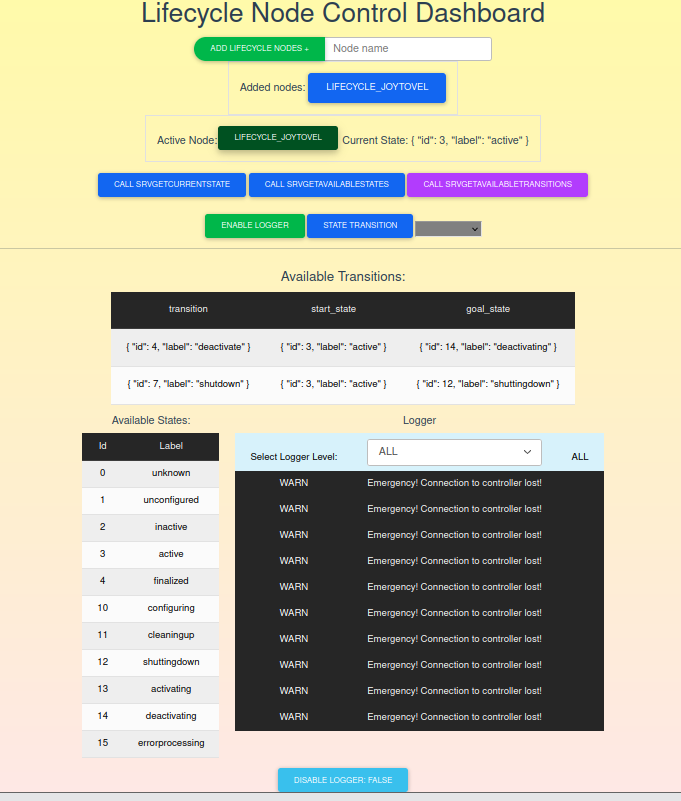
\includegraphics[width=0.95\textwidth]{"Bilder/lifecycle-dashboard.png"}
	\caption{Lifecycle Dashboard}
	\label{fig:Background:LifecycleDashboard}					
\end{figure}

\section{Integration}
\label{Implementierung:Integration}


	
		
		
	
	